%%% LaTeX template file for ZIB poster.
%%% ------------------------------------------------------------------------------------------------

\documentclass[pageborders]{zibposter}

% \usepackage[ngerman]{babel} % german (hyphenation... )
\usepackage[english]{babel} % english (hyphenation... )
\usepackage[utf8]{inputenc}
\usepackage{amsfonts}
\usepackage{booktabs}
\usepackage{caption}
\usepackage{amsmath}

\usepackage{tcolorbox}
\usepackage{xcolor}

\newtcolorbox{mybox}[3][]
{
  colframe = #2,
  colback  = #2!10!white,
  coltitle = black,  
  title    = \centering\normalsize #3,
  boxrule = 1pt,
  left=0pt,right=0pt,top=0pt,bottom=0pt,
  #1,
}

\newtheorem{theorem}{Theorem}
\newtheorem{definition}[theorem]{Definition}

\definecolor{mygray}{rgb}{0.6,0.6,0.6}

\usepackage{bbm}
\newcommand{\defi}{\stackrel{\scriptscriptstyle def}{=}}
\newcommand{\ones}{\mathbbm{1}}
\newcommand{\Rp}{\mathbb{R}_{\geq 0}} 
\newcommand{\R}{\mathbb{R}} 
\newcommand{\pol}{\mathcal{P}}
\newcommand{\D}{\mathcal{D}}
\newcommand{\norm}[1]{\| #1 \|}
\renewcommand{\epsilon}{\varepsilon}


% Tikz's shit

\usepackage{xparse}
\usepackage{tikz}			% To draw cats automatas etc etc
\usetikzlibrary{automata} 	% 
\usetikzlibrary{arrows} 	% Different types of arrows (e.g. inclusion)

\usetikzlibrary[shapes.arrows]
\usetikzlibrary{shapes.geometric}
\usetikzlibrary{backgrounds}
\usetikzlibrary{positioning}
\usetikzlibrary{calc}
\usetikzlibrary{intersections}
\usetikzlibrary{fadings}
\usetikzlibrary{decorations.footprints}
\usetikzlibrary{patterns}
\usetikzlibrary{shapes.callouts}
\usetikzlibrary{fit}

% Tikz Settings
\tikzset{->, >=stealth', shorten >=1pt, auto, node distance=1cm, semithick, baseline=(current bounding box.center)}


% Usage: \circled{1}[\leq] % it needs xparse and tikz
\newcommand*\circledaux[1]{\tikz[baseline=(char.base)]{
    \node[shape=circle,draw,inner sep=6pt] (char) {#1};}}

\NewDocumentCommand{\circled}{ m o }{%
    \IfNoValueTF{#2}{ \circledaux{#1} }{ \stackrel{\circledaux{#1}}{#2} }%
}

\DeclareMathOperator{\conv}{conv}

\newcommand{\bigo}[1]{O( #1 )}
\newcommand{\bigotilde}[1]{\widetilde{O}( #1 )}


\title{Faires Teilen des Internets \\ \en{Fair share of the Internet}}
%%% List the authors here.
\author{}
%%% List the cooperations and funding partners here.
\institute{}
% TODO

\newcommand{\en}[1]{{\color{gray}#1}}
\newcommand{\enLight}[1]{{\color{gray!40}#1}}

\begin{document}
	%%% Uncomment this to add the mathpluslogo
	%\mathpluslogo
	
	%%% This command creates your title.
	\maketitle % Create title

	%%% Here you can put your poster content.
	%%%
	%%% A box with a title is created by the following command:
	%%% \block{Title}{Content}
	%%% For a box without a titlebar just leave the title empty:
	%%% \block{}{Content}
	%%%
	%%% The content of a block allows regular latex code (with some exceptions).
	%%%
	%%% Blocks can span the width of the poster or can be placed inside columns.
	%%% Columns are defined like this:
	%%%
	%%% \begin{columns}
	%%% \column{.3} % this is a column spanning 30 percent of the width of the poster.
	%%% \block{Title1}{Content1}
	%%% \block{Title2}{Content2}
	%%% \column{.7} % this is a column spanning 70 percent of the width of the poster.
	%%% \block{Title3}{Content3}
	%%% \end{columns}
	%%%
	%%% At the very end of the poster creating process you should make sure that your
	%%% blocks at the end of the poster align. You can for example play around with
	%%% \vspace{2cm}
	%%%
	%%% Assuming your file is named 'poster.tex' you can compile it by opening a commandline,
	%%% navigating to the folder containing the file and typing
	%%%    pdflatex poster.tex
	%%%
	%%% A word to the papersize:
	%%% The frames at ZIB have b1paper format. Since the fontsizes and measurements should be uniform,
	%%% please use the following doumentclass and don't change neither the colorscheme nor
	%%% the fontsizes or fontfamilies:
	%%% \documentclass[grey,b1paper,fontserif]{zibposter}
	%%%
	%%% If you or your conference prefer a0paper or you like a different colorscheme
	%%% you can change these parameters in the documentclass.

    \block{Netzwerke! | \enLight{Networks!}}{
    \begin{minipage}[c]{0.52\linewidth}
        \begin{itemize}
            \item In gemeinsam genutzten Netzwerken wie dem Internet fordern Personen Informationen von Servern an, die Ihre bevorzugten Websites, Videos und Fotos über das Netzwerk senden.
            \item Die Informationen durchlaufen mehrere Verbindungen, bis sie ihr Ziel erreichen, und eine Verbindung kann jeweils nur eine begrenzte Menge an Informationen pro Sekunde senden.
          \item Der Weg, den die Informationen nehmen, ist für jeden Nutzer unterschiedlich.
            \item Wir können entscheiden, wie schnell wir die Daten jedes Servers an jeden Nutzer senden.
        \end{itemize}
      \vspace*{0.5cm}

      \begin{center}
      {\centering \LARGE WIR WOLLEN DIE GESCHWINDIGKEIT FAIR VERTEILEN!}
      \end{center}
          
      \end{minipage}%
      \begin{minipage}[c]{0.01\linewidth}
          \ 
      \end{minipage}%
      \begin{minipage}[c]{0.45\linewidth}
      \en{
          \begin{itemize}
            \item In shared networks, like the Internet, people request information to servers that send your favorite websites, videos, photos across the network.
            \item The information traverses several links until it reaches its destination, and a link can only send a limited amount of information per second.
            \item The path that the information follows is different for each user. 
            \item We can decide how fast we send the data of each server to each user. 
        \end{itemize}

      \vspace*{0.5cm}
      \begin{center}
      {\LARGE WE WANT TO ASSIGN SPEED FAIRLY!}
      \end{center}
      }
      \end{minipage}


      \begin{minipage}[c]{0.45\linewidth}
      \centering
      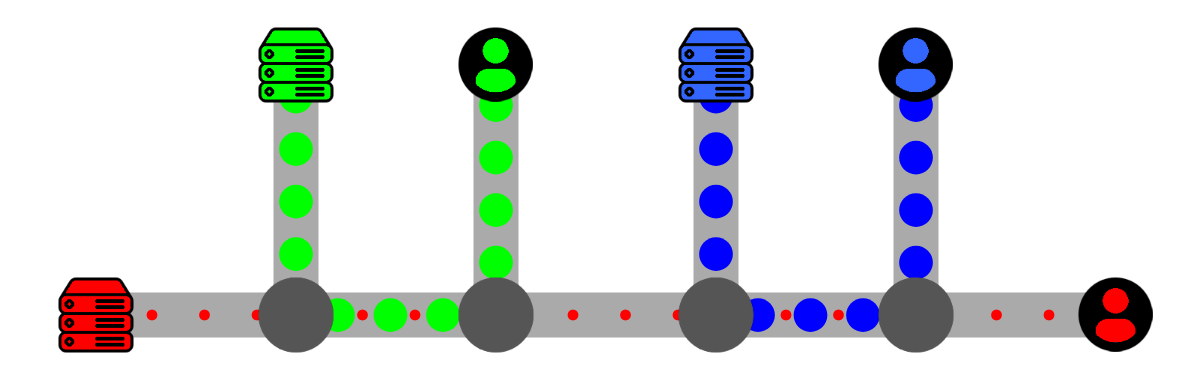
\includegraphics[width=0.95\linewidth] {graphics/axiom1.png}
      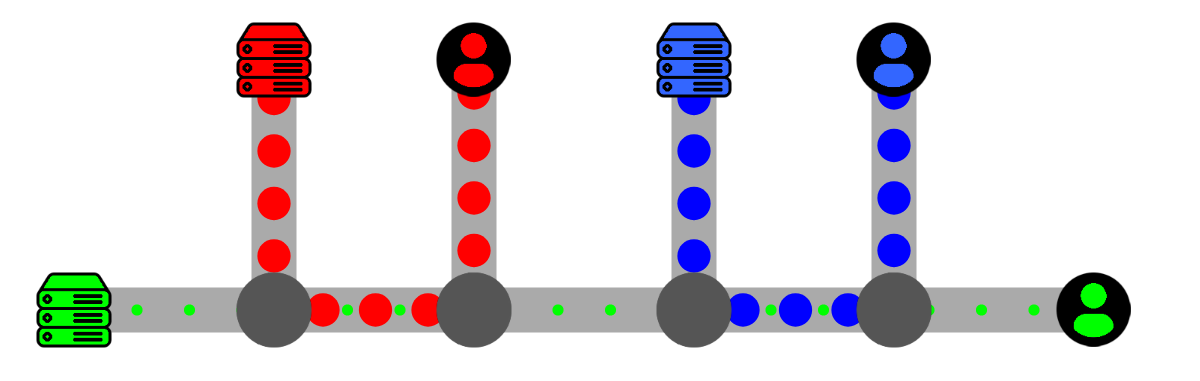
\includegraphics[width=0.95\linewidth] {graphics/axiom1b.png}
      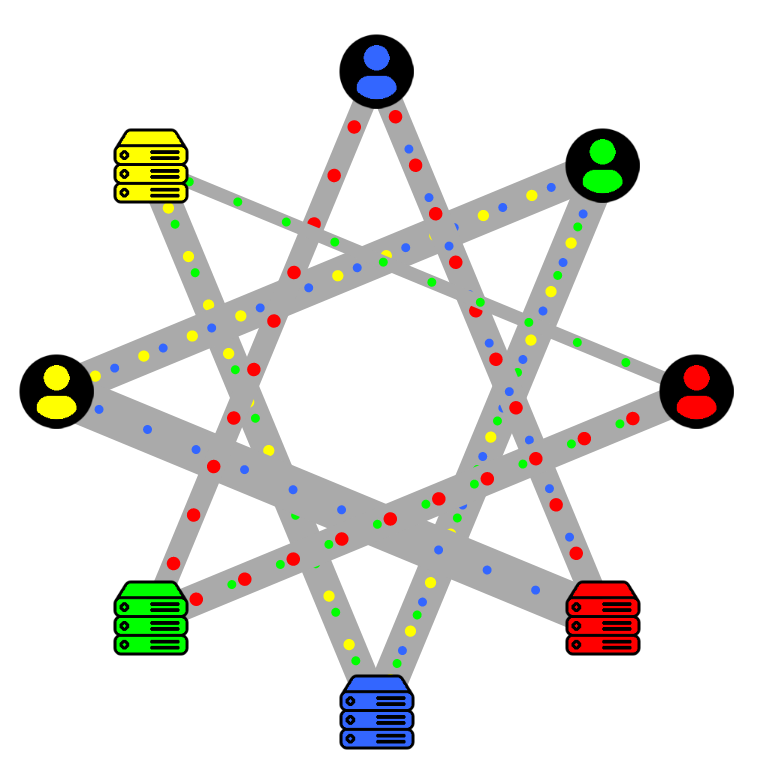
\includegraphics[width=0.95\linewidth] {graphics/octagon_white_background.png}

      \begin{minipage}[c]{0.8\linewidth}
      \begin{center}
          {\LARGE ES GIBT NUR EINEN WEG, DIE $4$ EIGENSCHAFTEN GLEICHZEITIG ZU ERFÜLLEN. VERSUCH ES SELBER.}

          \vspace*{0.5cm}
          \en{ \LARGE THERE IS ONLY ONE WAY OF SATISFYING THE $4$ PROPERTIES AT THE SAME TIME. TRY IT YOURSELF.}
      \end{center}
      \end{minipage}

      \end{minipage}%
      \begin{minipage}[c]{0.5\linewidth}
          \vspace*{0.8cm}
          \section*{Was bedeutet es, fair zu sein?}
          \begin{enumerate}
              \item[\circled{$1$}] \textbf{Wer du bist, sollte keine Rolle spielen! Keine Privilegien!} In den beiden ersten Netzwerken links sehen die fairen Verteilung gleich aus. Rot im ersten Netzwerk sollte dieselbe Verteilung erhalten wie Grün im zweiten Netzwerk.
            \item[\circled{$2$}] \textbf{Wenn wir die Geschwindigkeit für einen Nutzer erhöhen können, ohne dass jemand an Geschwindigkeit verliert, tun wir das.}
                  Bei der fairen Verteilung sollte es nicht passieren, dass ein Nutzer noch mehr Geschwindigkeit erhalten könnte, ohne die Geschwindigkeit anderer zu verringern. Das heißt, das Netz sollte voll genutzt werden!
              \item[\circled{$3$}] \textbf{Wie wir das Netzwerk teilen, sollte nicht davon abhängen, welche Einheiten wir verwenden!} Es wäre ziemlich seltsam, dass sich unsere Entscheidung ändert, nur weil wir uns entscheiden, statt Mb/s Nibbles pro Femtojahrhundert zu benutzen! (oder °C statt °F, wenn wir mit Temperaturen arbeiten).
              \item[\circled{$4$}] \textbf{Wenn wir weitere Einschränkungen hinzufügen, aber die vorherige faire Verteilung noch möglich ist, dann bleibt sie fair!} Wenn wir beispielsweise die Kapazität einer Verbindung reduzieren oder eine Verbindung entfernen, aber immer noch dieselbe Verteilung verwenden können, die wir zuvor getroffen haben, dann erachten wir sie weiterhin als fair. Allgemeiner gesagt: Wenn wir mehrere Optionen haben und eine davon als fair betrachten, dann wählen wir diese Verteilung immer noch als fair aus, wenn uns ein Szenario mit deutlich weniger Optionen präsentiert wird, wenn dies möglich ist.
          \end{enumerate}
          \en{
          \vspace*{-1.7cm}
          \section*{What does it mean to be fair?}
          \vspace*{-0.7cm}
          \begin{enumerate}
              \item[\circled{$1$}] \textbf{Who you are shouldn't matter! No privileges!} In the two first networks on the left, the fair assignments will look the same. Red in the first network should receive the same as green in the second network.
              \item[\circled{$2$}] \textbf{If we can give more speed without anyone losing any speed, we give more.} In the fair assignment it should not happen that one user could still receive more speed without decreasing the speed of others. That means, the network should be fully used!
              \item[\circled{$3$}] \textbf{How we share the network should not depend on which units we use!} It would be pretty strange that our decision changes just because instead of using Mb/s, we decide to use nibbles per femtocenturies or any other way to measure it! (or °C vs °F if we worked with temperature).
              \item[\circled{$4$}] \textbf{If we add more restrictions, but the previous fair assignment is still possible, then it is still fair!} If for example, we reduce the capacity of a link or we remove a link but we can still pick the fair choice we had made before, then we still pick it as fair. More in general, if we have some options and take one of them as fair, then we still select this assignment as fair if we are presented with a scenario with strictly fewer options, if we can.
          \end{enumerate}
          }
      \end{minipage}

    }

%\begin{table}
%    \centering
%    \caption{Comparison of algorithms for $\varepsilon$-approximating the $1$-fair packing problem and its dual. The work of one iteration is linear in $N$, the number of non-zero entries in $A$.}
%    \label{table:comparisons}


    \block{Verweise | \enLight{References}}{
      \nocite{*}
      \bibliographystyle{IEEEtran}
      \bibliography{bibfile}
 		}
	
	%%% --- begin content ------------------------------------------------------------------------------
% 	
% 	% TODO
% 	
% 	\block{Motivation}{
% 		Some short explanation of the goals or findings\\
% 		
% 		\begin{minipage}[t]{.3\linewidth}
% 			\begin{itemize}
% 				\item Point 1
% 				\item Point 2
% 				\item Point 3
% 				\item ...
% 				\item Point 41
% 				\item Point 42
% 				\item Point 43
% 			\end{itemize}
% 		\end{minipage}
% 		\begin{minipage}[t]{.7\linewidth}
% 			\begin{itemize}
% 				\item Goal 1
% 				\item Goal 2
% 				\item Goal 3
% 				\item ...
% 				\item Goal 41
% 				\item Goal 42
% 				\item Goal 43
% 			\end{itemize}
% 		\end{minipage}
% 	}
% 	
% 	\begin{columns}
% 		
% 		\column{.55}
% 		
% 		\block{A picture}{
% 			\begin{tikzfigure}[Ligand Excluded Surfance \cite{ref1}]
% 				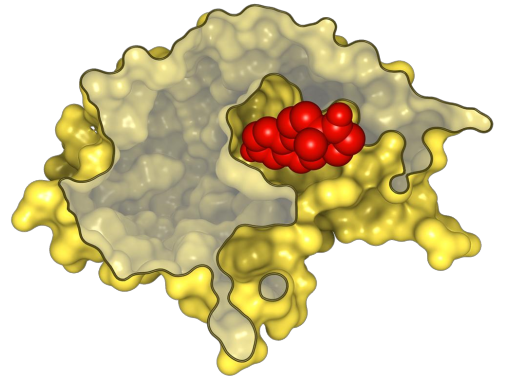
\includegraphics[width=0.7\linewidth]{graphics/demo/ligandExcludedSurface}
% 			\end{tikzfigure}
% 		}
% 		
% 		\block{Box Title}{
% 			Some text ...
% 
% 			\vspace*{180mm}
% 		}
% 		
% 		\column{.45}
% 		
% 		\block{Box Title}{
% 			A box with some latex math. First Euler's equation
% 			\[ e^{i\pi} + 1 =0 \]
% 			Second the geometric series
% 			\[ \sum_{k=0}^{n-1} q^k = \frac{1-q^n}{1-q} \]
% 		}
% 		
% 		\block{}{
% 			A box without a title.  A box without a title.
% 
% 			\vspace*{207mm}
% 		}
% 		
% 		\block{Font awesome}{
% 			Note that you can use fontawesome symbols:
% 			\begin{itemize}
% 				\item[\faUniversity] a university
% 				\item[\faBook] a book
% 				\item[\faGlobe] a globe
% 				\item[\faUsers] users
% 			\end{itemize}
% 			and much more, for references search the internet
% 		}
% 		
% 	\end{columns}
% 	
% 	\begin{columns}
% 		
% 		\column{.63}
% 		
% 		\block{Publications}{
% 			\begin{thebibliography}{9}
% 				\bibitem{ref1} N. Lindow, D. Baum, H.-C. Hege. Ligand Excluded Surface: A New Type of Molecular Surface.
% 				\textit{IEEE Transactions on Visualization and Computer Graphics,} Vol. 20, No. 12, pp. 2486--2495, 2014.    
% 			\end{thebibliography}
% 
% 			\vspace{20mm}
% 		}
% 		
% 		\column{.37}
% 		
% 		\block{Funded by}{			
% 			Our awesome partner and ...
% 			\hfill
% 			%
\includegraphics[height=2.4cm]{graphics/logos/ZIB-logo}
% 			\vspace{33mm}
% 		}
% 		
% 	\end{columns}
% 	
% 	%%% --- end content --------------------------------------------------------------------------------
\end{document}
